\documentclass{article}
\usepackage{graphicx}
\usepackage[top=10mm, bottom=25mm, left=30mm, right=30mm, includehead]{geometry}
\usepackage{fancyhdr}
\usepackage{mathptmx}
\usepackage{xcolor}
\let\negmedspace\undefined
\let\negthickspace\undefined
\usepackage{../gvv-book}
\usepackage{../gvv}
\usepackage{bm}
\usepackage{cite}
\usepackage{amsmath,amssymb,amsfonts,amsthm}
\usepackage{algorithmic}
\usepackage{textcomp}
\usepackage{listings}
\usepackage{enumitem}
\usepackage{mathtools}
\usepackage{gensymb}
\usepackage{comment}
\usepackage[breaklinks=true]{hyperref}
\usepackage{tkz-euclide}                                    
\usepackage[utf8]{inputenc}                           
\usepackage{color}                                            
\usepackage{array}                                            
\usepackage{longtable}       
\usepackage{calc}                                             
\usepackage{multirow}                       
\usepackage{hhline}                                           
\usepackage{ifthen}                                       
\usepackage{lscape}
\usepackage{tabularx}
\usepackage{float}
\usepackage{multicol}
%\usepackage{chngcntr}
%\counterwithout{figure}{section} 

\usepackage{caption}
\usepackage{subcaption}
\usepackage[T1]{fontenc}
\pagestyle{fancy}
\fancyhf{}
\date{}
\setlength{\headheight}{23.10004pt}

\fancypagestyle{plain}{
    \fancyhead[R]{\textit{$4^{th}$ International Conference on Recent Advances in Applied Mathematics (RAAM2026)\\ 6--8 July $2026$, Indian Institute of Technology, Hyderabad}}
    \renewcommand{\headrulewidth}{0pt}
    }
\onecolumn
\bibliographystyle{IEEEtran}
\numberwithin{equation}{section}
\numberwithin{figure}{section}
\renewcommand{\thetable}{\theenumi}

\title{\bfseries\large{A Logo for Narayanpal}}

\author{\underline{Subhodeep Chakraborty}\footnote{Department of Electrical Engineering, Indian Institute of Technology, Hyderabad}, Shiven Bajpai\footnote{Department of Artifical Intelligence, Indian Institute of Technology, Hyderabad} and G.V.V. Sharma\footnotemark[1]}

\begin{document}
\maketitle
%\vspace{-0.7cm}

%\begin{abstract}
This paper outlines a rigorous mathematical framework for generating a unique visual logo. Unlike conventional graphic design techniques that rely on free-form vector drawing, this approach derives a foundational geometric structure by linking a continuous-time signal's integral constraints to the analytic geometry of conic sections using matrix equations and decompositions. Specifically, we extract the decay parameters of an exponential signal by mapping them to the latus recta endpoints of a derived hyperbola. A precise truncation method based on decibel attenuation is then applied to the resulting infinite waveform to yield a bounded, aesthetic visual asset usable as a logo.
%\end{abstract}

%\vspace{0.1cm}
%\section*{Related Work and Summary}
%\footnote{A. Smith and J. Doe, \emph{J. of Visual Branding} \textbf{45}, 112 (2018).} 
Many companies map equations to their brand, such as Broadcom's sinc function and Cisco's discrete waveforms.  In graphics, mathematical frameworks utilise parametric primitives, double pendulum kinematics, or trigonometry for interactive patterns\footnote{P. Jha and B. B. Biswal, \emph{J. of Graphic Eng. and Design} \textbf{11}, 37 (2020).}\footnote{I. Staribratov and N. Manolova, \emph{Math. and Informatics} \textbf{65}, 72 (2022).}, or apply recursive sequences like the Golden Ratio or simplified 2:3:5 geometric ratios, to refine manually drawn curves.\footnote{M. Rizaldi and R. Anthonius, \emph{Adv. in Soc. Sci., Edu. and Hum. Res.} \textbf{502}, 21 (2020).} 
Despite these methodologies, a significant gap persists; existing mathematical framweorks ultimately require arbitrary aesthetic cropping in design software to finish the logo. 

This project overcomes this by introducing a purely mathematical approach from start to finish. Here, the logo's exact structural coordinates were analytically derived directly from signal processing constraints and eigenvalue decomposition, along with precise signal truncation derived from attenuation limits. Thus the final asset is fully mathematically generated.
% often translate mathematical functions directly into visual identities; for instance, Broadcom employs a stylized sinc function ($\operatorname{sinc}(x)$) to represent an ideal low-pass filter,\footnote{A. Smith and J. Doe, \emph{J. of Visual Branding} \textbf{45}, 112 (2018).} while Cisco merges a discrete digital waveform with the suspension geometry of the Golden Gate Bridge.\footnote{M. Weaver, \emph{Digital Waveforms in Art}, Tech Press (2020).} Foundational designs for consumer brands like Apple famously utilize the Fibonacci sequence and the Golden Ratio to achieve aesthetic perfection.\footnote{R. Evans et al., \emph{J. of Design Proportions} \textbf{22}, 15 (2015).} In academia, the National Institute of Advanced Studies (NIAS) bases its emblem on the \textit{śyenaciti}, an ancient geometric Vedic fire altar,\footnote{R. Narasimha, \emph{NIAS News} \textbf{8}, 2 (1999).} and computer science projects like MathSeer integrate equations directly into their user interface architectures.\footnote{R. Dmello, \emph{J. of Math UI} \textbf{4}, 102 (2019).} 

%Building upon this legacy of using proportional overlays or explicit functional graphs, our paper proposes a novel synthesis. Instead of relying on parametric primitives or isolated formulas, we derive a logo's exact structural coordinates by leveraging continuous-time signal processing constraints alongside eigenvalue decomposition. Our method mandates that the visual shape is the strict analytical outcome of a converging area integral.
%\vspace{0.1cm}
The logo's underlying structure is defined by the function $f(t) = e^{-at}u(t) + e^{bt}u(-t)$. 
which is the probability density function of an exponential conditionally Gaussian random variable
\footnote{G. V. V. Sharma, U. B. Desai, and S. N. Merchant, \emph{IEEE Trans. Wireless Commun.} \textbf{10}, 27 (2011).}.
%. A conditionally Gaussian random variable
%with parameters a, b > 0 is defined as Z ∼N(aA,bA) where A is a random variable. In this paper, we assume that A is exponentially distributed with parameter c. We refer to such variables as 

	
The parameters $(a,b)$ are derived by enforcing a constraint for unit area, yielding the conic section $ab - a - b = 0$. By expressing this conic in the standard quadratic form $\text{g}(\vec{x}) = \vec{x}^\text{T}\vec{Vx} + 2\vec{u}^\text{T}\vec{x} + f$ and performing eigendecomposition, we apply affine transformations to map the hyperbola into a standard coordinate system. The parameters $(a,b)$ are then explicitly chosen as the valid endpoints of the latus recta of this conic, yielding a precise solution (see \figref{fig:hyper}).% $\vec{\hat{x}}_1 = \myvec{2+\sqrt{2} \\ \sqrt{2}}$. 
%\vspace{0.1cm}
To serve as a practical logo, the graph was truncated. Rather than arbitrary cropping, a $-30$dB amplitude attenuation threshold was enforced to derive theoretical truncation bounds $t_1$ and $t_2$ precisely. The resulting bounded graph in \figref{fig:pexp} was taken as the final mathematically synthesised logo.

%\vfill

\begin{figure}[H]
	\centering
    \begin{subfigure}[b]{0.45\textwidth}
        \centering
	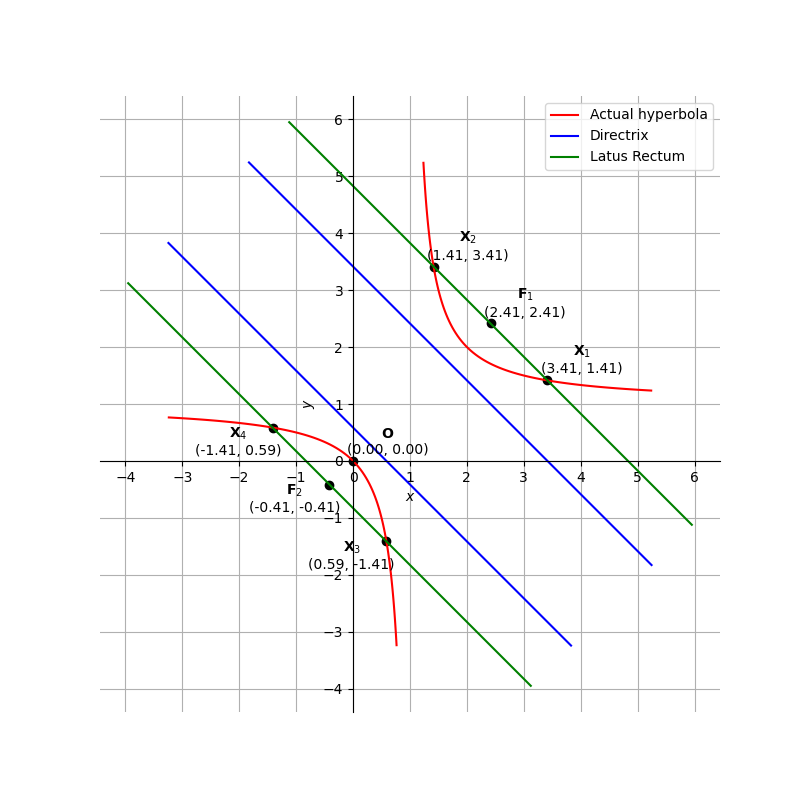
\includegraphics[width=0.65\columnwidth]{../figs/Hyperbola.png}
    \caption{Derived: $a=2+\sqrt{2}$, $b=2$}
	\label{fig:hyper}
    \end{subfigure}
    \hfill
    \begin{subfigure}[b]{0.45\textwidth}
        \centering
	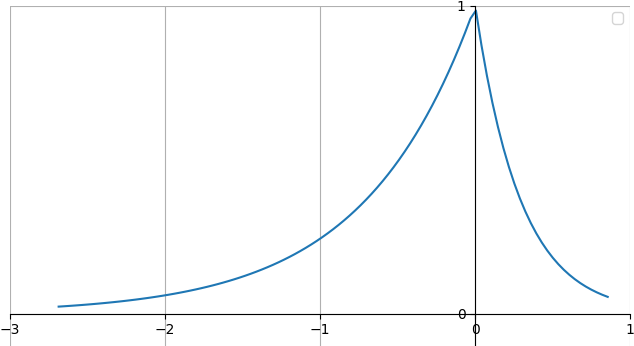
\includegraphics[width=\columnwidth]{../figs/trunc1.png}
	\caption{Truncated at $t_1\approx -2.6874$ and $t_2\approx 0.8550$}
	\label{fig:pexp}
    \end{subfigure}
	%\caption{The final truncated logo generated from the derived parameters $(a,b)$.}
%	\label{fig:Truncation}
\end{figure}

\iffalse
\begin{figure}[H]
    \centering
    \begin{subfigure}[b]{0.45\textwidth}
        \centering
        %\rule{\linewidth}{4cm}
        \includegraphics[width=0.8\textwidth]{topview.jpg}
        \caption{Top view}
    \end{subfigure}
    \hfill
    \begin{subfigure}[b]{0.45\textwidth}
        \centering
        %\rule{\linewidth}{4cm}
        \includegraphics[width=0.8\textwidth]{side view.jpg}
        \caption{Side view}
    \end{subfigure}
    \caption{Circuit}
    \label{fig:circuit}
\end{figure}
\fi
\end{document}
